\section{Jatkuvuuden käsite} \label{jatkuvuuden käsite}
\alku

Funktion jatkuvuuden ongelma tulee eteen niinkin yksinkertaisessa tehtävässä kuin funktion
arvon numeerisessa määrittämisessä, eli numeerisessa funktioevaluaatiossa. Tarkastellaan Luvun 
\ref{käänteisfunktio} Esimerkin \ref{algebrallinen käänteisfunktio} käänteisfunktiota, 
joka nyt kirjoitettakoon muotoon
\[
y=f(x) \ \ekv \ y^5+3y=x, \quad x\in\R.
\]
Tehtävänä olkoon laskea likimäärin luku $a=f(\pi)$, eli evaluoida $f$ numeerisesti $\pi$:ssä. 
Tähän itse asiassa sisältyy kaksi numeerista ongelmaa: Ensinnäkin luvulle $\pi$ ei ole olemassa
'tarkkaa' numeerista arvoa, ja toiseksi yhtälöä ei yleensä voi ratkaista $y$:n suhteen
tarkasti, vaikka $x$ olisi rationaaliluku. Käytännössä menetellään (laskin/tietokone 
menettelee) seuraavasti: Valitaan $\pi$:lle edustaja $x_n$ rationaalilukujonosta $\{x_n\}$,
jolle pätee $x_n\rightarrow \pi$. Lasketaan $a_n=f(x_n)$ likimäärin käyttämällä jotakin
numeerista algoritmia yhtälön $y^5+y=x_n$ ratkaisuun. Algoritmi tuottaa käytännössä
rationaalilukujonon $\{b_k\}$, jolle pätee $b_k \kohti a_n$ kun $k\rightarrow\infty$. Poimitaan
tästä jonosta luvun $a_n$ likiarvoksi $b_m$ jollakin $m$ (esim.\ $m=10$), ja ilmoitetaan
lopputuloksena tämän luvun likiarvo äärellisenä desimaalilukuna (katkaistuna tai pyöristettynä
liukulukuna). 

Jos em.\ laskussa ei huomioida numeerisia pyöristysvirheitä liukulukulaskennassa, niin 
lopputuloksen $b_m$ virhe koostuu kahdesta osasta:
\[
b_m-f(\pi)\,=\,[b_m-f(x_n)]+[f(x_n)-f(\pi)].
\]
Tässä ensimmäinen osa on approksimaation $b_m \approx f(x_n)$ virhe, eli kyse on yhtälön
$y^5+3y=x_n$ ratkaisualgoritmin tarkkuudesta. Virheen jälkimmäisessä osassa sen sijaan on kyse,
paitsi approksimaation $x_n \approx x$ tarkkuudesta, myös funktiosta $f$: Kyse on funktion 
j\pain{atkuvuudesta}. Kvalitatiivisesti väittämä '$f$ on jatkuva $x$:ssä' tarkoittaa, että
funktioevaluaatio $x \map f(x)$ on luotettava, kun muuttujalle sallitaan pieni vaihtelu, ts.\
pätee
\[
x_n\approx x \ \impl \ f(x_n)\approx f(x).
\]

Em.\ funktion tapauksessa jatkuvuuskysymys ratkeaa seuraavasti: Koska
\[
\begin{cases}
a^5+a=\pi, \\
a_n^5+a_n=x_n,
\end{cases}
\]
saadaan vähennyslaskulla (vrt. Luvun \ref{käänteisfunktio} tarkastelut)
\[
(a-a_n)(a^4+a^3a_n+a^2a_n^2+aa_n^3+a_n^4+3)=\pi-x_n.
\]
Tässä voidaan turvallisesti olettaa, että $a,a_n \ge 0$, joten seuraa
\[
\abs{a_n-a}\le \tfrac{1}{3}\abs{x_n-\pi}\,\ \ekv\,\ 
\abs{f(x_n)-f(\pi)}\le\tfrac{1}{3}\abs{x_n-\pi}.
\]
Jatkuvuudelle on näin saatu jopa kvantitatiivinen varmistus: Approksimaation $f(x_n)$ $\approx$
$f(\pi)$ virhe on enintään kolmasosa approksimaation $x_n\approx \pi$ virheestä. 

Esimerkki johdattaa seuraavaan funktion jatkuvuuden määritelmään (vaihtoehtoinen määritelmä 
jäljempänä).
\begin{Def} \vahv{(Jatkuvuus: jonokriteeri)}\ \label{funktion jatkuvuus}
\index{jatkuvuus (yhden muuttujan)|emph} \index{epzy@epäjatkuvuus (funktion)|emph}
Funktio $f:\DF_f\rightarrow\R,\ \DF_f\subset\R$, on \kor{jatkuva} (engl.\ continuous, ruots.\ 
kontinuerlig) \kor{pisteessä} $a\in\DF_f$ (tai $a$:ssa), jos kaikille reaalilukujonoille
$\seq{x_n}$ pätee
\[
x_n\in\DF_f\ \forall n\,\ \ja\,\ x_n \kohti a\,\ \impl\,\ f(x_n) \kohti f(a).
\]
Jos $f$ ei ole jatkuva pisteessä $a\in\DF_f$, niin $f$ on \kor{epäjatkuva}
(engl.\ discontinuous) pisteesä $a$.
\end{Def}
\begin{Exa} \label{epäjatkuva funktio} Funktio \
$\D f(x)= \begin{cases} \,x-1, &\text{jos}\ x<\pi \\ \,x, &\text{jos}\ x\ge\pi \end{cases}$
\vspace{1mm}\newline
on epäjatkuva pisteessä $x=\pi$, sillä jos $x_n \kohti \pi$ ja $x_n<\pi\ \forall n$, niin
$f(x_n)=x_n-1 \kohti \pi-1 \neq f(\pi)=\pi$. Muissa pisteissä $f$ on jatkuva, sillä jos esim.\
$a<\pi$ ja $x_n \kohti a$, niin jostakin indeksistä $N$ eteenpäin on $\abs{x_n-a}<\pi-a$ 
(lukujonon suppenemisen määritelmässä valittu $\eps=\pi-a$), jolloin on erityisesti 
$x_n-a < \pi-a\ \ekv\ x_n<\pi$, kun $n>N$. Tällöin on $f(x_n)=x_n-1,\ n>N$ ja siis
$f(x_n) \kohti a-1=f(a)$. \loppu
\end{Exa}
\begin{Exa} Olkoon $\DF_f=\{a\}$ ($a\in\R$) ja $f(a)=c\in\R$. Määritelmän
\ref{funktion jatkuvuus} mukaisesti $f$ on jatkuva pisteessä $a$\,(!). Yleisemmin
reaalifunktio on jatkuva jokaisessa määrittelyjoukkonsa nk.\ \kor{eristetyssä pisteessä},
ks.\ Harj.teht.\,\ref{H-V-1: eristetty piste}. \loppu
\end{Exa}
Jatkuvuus voidaan määritellä myös suoraan vetoamatta lukujonoihin, jolloin määritelmästä tulee 
lukujonon suppenemisen määritelmää (Määritelmä \ref{jonon raja}) muistuttava. Vaihtoehtoinen
määritelmä on seuraava.
\begin{Def} \vahv{(Jatkuvuus: $(\eps,\delta)$-kriteeri)}\ \label{vaihtoehtoinen jatkuvuus}
\index{jatkuvuus (yhden muuttujan)|emph}
Funktio $f:\DF_f\kohti\R,\ \DF_f\subset\R$, on jatkuva pisteessä $a\in\DF_f$, jos jokaisella
$\eps>0$ on olemassa $\delta>0$ siten, että jokaisella $x\in\R$ pätee
\[
x\in\DF_f\,\ \ja\,\ \abs{x-a}<\delta\,\ \impl\,\ \abs{f(x)-f(a)}<\eps.
\]
\end{Def}
Määritelmiä \ref{funktion jatkuvuus} ja \ref{vaihtoehtoinen jatkuvuus} verrattaessa ei näytä
aivan ilmeiseltä, että pätee (ks.\ todistus luvun lopussa)
\begin{*Lause} \label{jatkuvuuskriteerien yhtäpitävyys} Jatkuvuuden määritelmät
\ref{funktion jatkuvuus} ja \ref{vaihtoehtoinen jatkuvuus} ovat yhtäpitävät.
\end{*Lause} 
\jatko\jatko \begin{Exa} (jatko) Jos $a\neq\pi$, niin esimerkin funktiolle pätee
\[
\abs{f(x)-f(a)}=\abs{x-a}, \quad \text{kun}\ \abs{x-a}<\abs{\pi-a},
\]
joten Määritelmän \ref{vaihtoehtoinen jatkuvuus} ehto on voimassa, kun valitaan
$\delta=\min\{\eps,\abs{\pi-a}\}>0$. Siis $f$ on jatkuva pisteissä $a\neq\pi$ Määritelmän
\ref{vaihtoehtoinen jatkuvuus} mukaisesti. \loppu
\end{Exa} \seur
\begin{Exa} Näytä, että $f(x)=x^2$ on jatkuva jokaisessa pisteessä $a\in\R$
käyttäen jatkuvuuden a) jonokriteeriä,\, b) $(\eps,\delta)$-kriteeiä.
\end{Exa}
\ratk \ a) Määritelmän \ref{funktion jatkuvuus} mukainen jatkuvuus on seuraus Lauseesta
\ref{raja-arvojen yhdistelysäännöt}:
\[
x_n \kohti a \qimpl x_n^2 \kohti a^2\,\ \impl\,\ f(x_n) \kohti f(a).
\]
b) Jos $a\in\R$ ja $\abs{x-a} \le 1$, niin kunta-algebran ja kolmioepäyhtälön nojalla
\begin{align*}
\abs{f(x)-f(a)}\,=\,\abs{x-a}\abs{x+a}\,
                &=\,\abs{x-a}\abs{2a+(x-a)} \\
                &\le\,\abs{x-a}(2\abs{a}+\abs{x-a})\,
                 \le\,\abs{x-a}(2\abs{a}+1).
\end{align*}
Näin ollen jos $\eps>0$, niin pätee $\abs{f(x)-f(a)}<\eps$ aina kun
$\abs{x-a}<\delta=\min\{1,\eps/(2\abs{a}+1)\}$ (jolloin myös $\abs{x-a}<1$). Koska tässä on
$\delta>0$ aina kun $\eps>0$, niin $f$ on jatkuva $a$:ssa
Määritelmän \ref{vaihtoehtoinen jatkuvuus} mukaisesti. \loppu

Jatkuvuuden määrittely jonokriteerillä (Määritelmä \ref{funktion jatkuvuus}) on kätevää
monissa teoreettisissa tarkasteluissa, jotka tällä tavoin palautuvat suppenevien
lukujonojen teoriaan. (Tämä teoria on kylläkin tunnettava, mitä voi pitää myös
haittapuolena.) Määritelmä \ref{vaihtoehtoinen jatkuvuus} on jatkuvuuden perinteisempi
'koulumääritelmä'. Tämä on usein Määritelmää \ref{funktion jatkuvuus} selkeämpi silloin kun
halutaan selvittää, miltä jatkuvat funktiot 'näyttävät'. Esimerkiksi seuraava usein käytetty
tulos, joka kertoo jatkuvan funktion 'jäykkyydestä', on tästä määritelmästä helppo johtaa.
Todistus jätetään harjoitustehtäväksi (Harj.teht.\,\ref{H-V-1: todistuksia}a).
\begin{Prop} \label{jatkuvan funktion jäykkyys} Jos $f$ on jatkuva pisteessä $a$ ja $f(a)>0$
($f(a)<0$), niin $\exists\delta>0$ siten, että $f(x)>0$ ($f(x)<0$) aina kun 
$x\in(a-\delta,a+\delta) \cap \DF_f\,$.
\end{Prop}

Jatkuvuus yksittäisessä pisteessä voidaan laajentaa koskemaan joukkoa $A\subset\DF_f$\,:
Funktio on jatkuva $A$:ssa, jos se on jatkuva $A$:n jokaisessa pisteessä. 
Jatkuvuustarkasteluille on kuitenkin tyypillistä, että tarkastelu rajoittuu \pain{välille} 
$A\subset\DF_f$ siten, että funktion ominaisuuksilla välin ulkopuolella ei ole lainkaan
merkitystä. Sen vuoksi on tapana asettaa mainitusta yleisestä säännöstä hieman poikkeava
\begin{Def} (\vahv{Jatkuvuus välillä}) \label{jatkuvuus välillä}
\index{jatkuvuus (yhden muuttujan)!a@välillä|vahv}
Funktio $f:\DF_f\kohti\R,\ \DF_f\subset\R$, on \kor{jatkuva välillä} $A\subset\DF_f$, jos
jokaisella $x \in A$ ja jokaiselle reaalilukujonolle $\seq{x_n}$ pätee
\[
x_n \in A\ \ja\ x_n \kohti x\,\ \impl\,\ f(x_n) \kohti f(x).
\]
\end{Def}
Tämän mukaisesti jatkuvuus välillä $A$ tarkoittaa samaa kuin Määritelmän
\ref{funktion jatkuvuus} mukainen jatkuvuus $A$:n jokaisessa pisteessä siinä tapauksessa, että
funktion määrittelyjoukko rajataan väliksi $A$. (Jatkuvuuden vaihtoehtoisessa määritelmässä
\ref{vaihtoehtoinen jatkuvuus} korvataan ehto $\,x\in\DF_f\,$ ehdolla $x\in\DF_f \cap A$.)
Jatkuvuus välillä määritellään siis jatkuvuutena 'sisältä päin' ko.\ joukossa. Jos väli on
avoin, ei tämä rajaus ole tarpeen, sillä jos $x\in(a,b)=A$ ja $x_n \kohti x$, niin jollakin $N$
pätee $x_n \in A\ \forall n>N$ (Määritelmä \ref{jonon raja}, $\eps=\min\{x-a,b-x\}>0$) eli
määritelmän ehto toteutuu indeksistä $N$ eteenpäin joka tapauksessa. Sen sijaan jos väli on
suljettu, on ehdolla $x_n \in A$ merkitystä välin päätepisteissä (ei sisäpisteissä).
\jatko\jatko \jatko \begin{Exa} (jatko) Jos $b>\pi$, on esimerkin funktio $f$ jatkuva välillä
$[\pi,b]$ (Määritelmä \ref{jatkuvuus välillä}) vaikka $f$ ei ole jatkuva pisteessä $\pi$
(Määritelmä \ref{funktion jatkuvuus}). Jos $a<\pi$, on $f$ jatkuva välillä $[a,\pi)$ mutta ei
välillä $(a,\pi]$. \loppu
\end{Exa} \seur\seur
\begin{Exa} \label{Dirichlet'n funktio} \index{Dirichleta@Dirichlet'n funktio}
Funktio $\D
f(x)=\begin{cases}
     \,1, \ &\text{ jos } x\in\Q,  \\
     \,0, &\text{ jos } x\in\R, \ x\notin\Q
     \end{cases}$ \vspace{2mm}\newline
on esimerkki 'patologisesta' funktiosta, joka on määritelty koko $\R$:ssä, mutta joka ei ole 
missään pisteessä jatkuva. Funktion nimi on \kor{Dirichlet'n funktio}.  \loppu
\end{Exa}

\subsection*{Jatkuvien funktioiden yhdistely}

Esimerkin \ref{Dirichlet'n funktio} vastapainoksi voidaan kysyä, millaiset 'normaalit' funktiot 
tyypillisesti ovat jatkuvia. Ensimmäinen tuntuma näihin saadaan yhdistelemällä yksinkertaisia 
funktioita peruslaskutoimituksilla Määritelmän \ref{funktioiden yhdistelysäännöt} mukaisesti.
Koska funktion jatkuvuudessa on viime kädessä kyse lukujonon $\seq{f(x_n)}$ suppenemisesta,
on seuraava lause välitön seuraus Lauseesta \ref{raja-arvojen yhdistelysäännöt}
(Harj.teht.\,\ref{H-V-1: todistuksia}b).
\begin{Lause} (\vahv{Jatkuvuuden yhdistelysäännöt}) \label{jatkuvuuden yhdistelysäännöt}
\index{jatkuvuus (yhden muuttujan)!b@yhdistelysäännöt|emph}
Jos $f:\DF_f\kohti\R$ on jatkuva pisteessä $x\in\DF_f$, niin $\lambda f$ on jatkuva $x$:ssä 
$\forall\lambda\in\R$. Jos lisäksi $x\in\DF_g$ ja $g:\DF_g\kohti\R$ on jatkuva pisteessä $x$,
niin $f+g$ ja $fg$ ovat jatkuvia $x$:ssä. Jos edelleen $g(x)\neq 0$, niin myös $f/g$ on
jatkuva $x$:ssä.
\end{Lause}
\begin{Exa} Jokainen polynomi tai rationaalifunktio voidaan määritellä palautuvasti
algebrallisena yhdistelmänä perusfunktioista $f_0(x)=1$ ja $f_1(x)=x$. Koska nämä ovat
ilmeisen jatkuvia $\R$:ssä, niin päätellään Lauseesta \ref{jatkuvuuden yhdistelysäännöt},
että jokainen polynomi on jatkuva $\R$:ssä ja jokainen rationaalifunktio
määrittelyjoukossaan, eli muualla kuin nimittäjänsä nollakohdissa. \loppu 
\end{Exa}
\begin{Exa} \label{trig yhdistely} Jos pidetään tunnettuna, että trigonometriset funktiot
$\sin$ ja $\cos$ ovat jatkuvia $\R$:ssä, niin Lauseen \ref{jatkuvuuden yhdistelysäännöt}
perusteella funktiot $\tan=\sin/\cos$ ja $\cot=\cos/\sin$ ovat samoin jatkuvia koko
määrittelyjoukossaan. \loppu 
\end{Exa}
\begin{Lause} (\vahv{Yhdistetyn funktion jatkuvuus}) \label{yhdistetyn funktion jatkuvuus}
\index{jatkuvuus (yhden muuttujan)!c@yhdistetyn funktion|emph}
Jos $g$ on jatkuva pisteessä $x\in\DF_g$, $g(x)\in\DF_f$ ja $f$ on jatkuva pisteessä $g(x)$,
niin yhdistetty funktio $f\circ g$ on jatkuva $x$:ssä.
\end{Lause}
\tod Koska $\,x_n\in\DF_{f \circ g}\ \ekv\ x_n\in\DF_g\,\wedge\,g(x_n)\in\DF_f$, niin
jonokriteerin avulla päätellään:
\begin{align*}
x_n \in\DF_{f\circ g}\ \ja\ x_n \kohti x 
           &\qimpl g(x_n)\in\DF_f\ \ja\ x_n\in\DF_g\ \ja\ x_n \kohti x \\
           &\qimpl g(x_n)\in\DF_f\ \ja\ g(x_n) \kohti g(x) \\
           &\qimpl f(g(x_n)) \kohti f(g(x)). \quad\loppu
\end{align*}
\begin{Exa} \label{itseisarvon jatkuvuus} Näytä, että jos $f$ on jatkuva $x$:ssä, niin myös
$\abs{f}$ on jatkuva $x$:ssä. 
\end{Exa}
\ratk Funktio $g(x)=\abs{x}$ on helposti osoitettavissa jatkuvaksi $\R$:ssä suoraan
jatkuvuuden määritelmistä (tai vedoten Propositioon \ref{jatkuvuuspropositio} alla), joten
Lauseen \ref{yhdistetyn funktion jatkuvuus} nojalla yhdistetty funktio 
$(g \circ f)(x) = \abs{f(x)}$ on jatkuva jokaisessa pisteessä, jossa $f$ on jatkuva. \loppu

Jatkuvuuden periytyvyyden p\pain{aloittain} (eli eri väleillä erilaisilla laskusäännöillä)
määritellyn funktion osalta ratkaisee
(Harj.teht.\,\ref{H-V-1: todistuksia}c; vrt.\ myös Esimerkki \ref{epäjatkuva funktio} edellä).
\begin{Prop} \label{jatkuvuuspropositio}
Olkoon $f_1$ ja $f_2$ jatkuvia avoimella välillä $(a,b)$ ja
\[
f(x) = \begin{cases} 
       \,f_1(x), &\text{kun}\ x \in (a,c), \\ 
       \,k, &\text{kun}\ x=c, \\ 
       \,f_2(x), &\text{kun}\ x \in (c,b),
       \end{cases} 
\]
missä $a<c<b$. Tällöin $f$ on jatkuva $c$:ssä täsmälleen kun $\,f_1(c)=f_2(c)=k$. 
\end{Prop}
\begin{Exa} Funktio
\[ f(x) = \begin{cases}
          \ x+a,\ &\text{kun}\ x \le a, \\ -(x+1)^2,\ &\text{kun}\ x > a 
          \end{cases} 
\] 
on polynomi $f_1(x)=x+a$ välillä $(-\infty,a)$ ja polynomi $f_2(x)=-(x+1)^2$ välillä
$(a,\infty)$, joten näillä väleillä funktio on jatkuva. Proposition \ref{jatkuvuuspropositio}
mukaan ehto funktion jatkuvuudelle pisteessä $x=a$ (ja siis ehto jatkuvuudelle koko $\R$:ssä)
on
\[
f_1(a)=f_2(a) \qekv a^2+4a+1=0 \qekv a = -2 \pm \sqrt{3}. \loppu
\]
\end{Exa}

\subsection*{Funktio $f(x) = \sqrt[m]{x}$}
\index{jatkuvuus (yhden muuttujan)!d@funktion $\sqrt[m]{x}$|vahv}

Osoitetaan seuraavaksi, että funktio $f:[0,\infty)\rightarrow [0,\infty)$, joka määritellään
\[
f(x)=x^{1/m}=\sqrt[m]{x},\quad m\in\N, \ m\geq 2
\]
on koko määrittelyvälillään jatkuva (kuvassa $f(x)$, kun $m=8$).
\begin{figure}[H]
\begin{center}
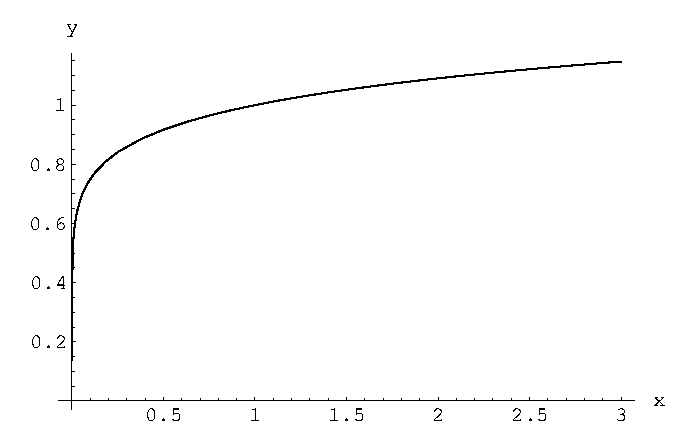
\epsfig{file=plots/8throotx.eps}
%\caption{$y=\sqrt[8]{x}$}
\end{center}
\end{figure}
Aloitetaan pisteestä $x=0$, joka on jatkuvuuden kannalta kriittisin (vrt. kuva). Koska f on 
aidosti kasvava (ks.\ Luku \ref{käänteisfunktio}, Esimerkki \ref{x^m:n käänteisfunktio}),
niin jokaisella $a>0$ pätee
\[
0 \le x < a^m\ \ekv\ 0 \le f(x) < f(a^m) = a.
\]
Jos nyt $x_n\geq 0$ ja $x_n\rightarrow 0$, niin jokaisella $\eps>0$ $\exists N\in\N$ siten,
että pätee
\[
n>N \ \impl \ 0 \le x_n < \eps^m \ \impl\ 0 \le f(x_n) < \eps.
\]
Näin ollen lukujono $\{f(x_n)\}$ on suppeneva ja $f(x_n) \kohti 0=f(0)$, joten $f$ on jatkuva 
$0$:ssa.

Muualla kuin origossa $f$:n jatkuvuus voidaan päätellä kunta-algebran avulla: Jos 
$x_n \ge 0$ ja $x_n \kohti x>0$, niin merkitsemällä $y=f(x)$, $y_n=f(x_n)$ seuraa
\[
x-x_n \,=\, y^m-y_n^m \,=\, (y-y_n)(y^{m-1}+y^{m-1}y_n+\cdots +y_n^{m-1}).
\]
Tässä on $y_n \ge 0$, $y>0$, joten päätellään
\[
\abs{x-x_n}\,\ge\,\abs{y-y_n}y^{m-1} \,\ \ekv\,\ \abs{y-y_n}\,\le\,y^{1-m}\abs{x-x_n}.
\]
Näin ollen $x_n \kohti x \ \impl\ y_n \kohti y$, eli $f$ on jatkuva pisteessä $x$.
\begin{Exa} \label{epsilon ja delta} Olkoon $\eps = 10^{-6}$. Määritä suurin $\delta$ siten,
että Määritelmän \ref{vaihtoehtoinen jatkuvuus} ehto toteutuu funktiolle $f(x)=\sqrt[8]{x}$
pisteessä $x=0$.
\end{Exa}
\ratk Koska $f$ on aidosti kasvava välillä $[0,\infty)=\DF_f$, niin $\forall x\in\DF_f$ pätee
$|f(x)-f(0)|=\sqrt[8]{x} < \eps\ \ekv\ 0 \le x < \eps^8\ \ekv\ x\in(-\eps^8,\eps^8)\cap\DF_f$.
Siis $\,\delta_{max} = \eps^8 = 10^{-48}$. \loppu

Funktion $f(x)=x^{1/m}$ jatkuvuuden tultua todetuksi seuraa Lauseesta 
\ref{yhdistetyn funktion jatkuvuus} ja funktion $g(x)=\abs{x}$ jatkuvuudesta, että yhdistetty 
funktio $(f\circ g)(x) = \abs{x}^{1/m}$ on jatkuva koko määrittelyjoukossaan ($= \R$). Kun
huomioidaan myös Lause \ref{jatkuvuuden yhdistelysäännöt}, niin seuraa
\begin{Prop} \label{potenssifunktion jatkuvuus}
Funktio $f(x)=\abs{x}^\alpha$, $\alpha=p/q\in\Q$ on koko määrittelyjoukossaan ($\DF_f=\R$ jos
$\alpha>0$, $\DF_f=\{x\in\R \mid x \neq 0\}$ jos $\alpha \leq 0$) jatkuva.
\end{Prop}
Lauseiden \ref{jatkuvuuden yhdistelysäännöt}--\ref{yhdistetyn funktion jatkuvuus}, Proposition
\ref{potenssifunktion jatkuvuus} ja Esimerkkien \ref{trig yhdistely} ja
\ref{itseisarvon jatkuvuus} perusteella voidaan vetää se yleisempi johtopäätös, että kaikki
toistaiseksi tunnetut 'yhden lausekkeen' funktiot ovat jatkuvia koko määrittelyjoukossaan (!).
\begin{Exa} Ilman tapauskohtaista tarkastelua voidaan esimerkiksi seuraavat funktiot
päätellä jatkuviksi määrittelyjoukkonsa jokaisessa pisteessä:
\[
\sqrt[3]{\abs{1-\sqrt{x}\,}}\,, \quad 
\sqrt[6]{\frac{1+\sqrt{x}}{2-x^2}}\,, \quad
\frac{|\sin x|^{3/4}}{x-\pi}\,, \quad 
\frac{\cot x}{\sqrt[4]{x+50\cos(\tan x)}}\,. \loppu
\]
\end{Exa}

\subsection*{Jatkuvien funktioiden päälauseet}

Tässä osaluvussa esitetään kolme matemaattisen analyysin keskeistä lausetta, jotka kaikki
koskevat suljetulla välillä jatkuvia funktioita. Ensimmäinen lauseista on myös ensimmäinen
yhden reaalimuuttujan funktioita koskevista \kor{väliarvolauseista}, joita on kaikkiaan kolme.
(Muut kaksi esitetään myöhemmin.) Tässä esitettävistä päälauseista jälkimmäiset kaksi ovat
erikoistapauksia yleisemmistä väittämistä, jotka perustuvat jatkuvuuden syvällisempään
logiikkaan. Näiden todistuksia ei vielä esitetä, vaan lauseet muotoillaan ja todistetaan
jäljempänä Luvussa \ref{jatkuvuuden logiikka} tässä esitettyä yleisemmässä muodossa. 
 
Tarkastellaan suljetulla välillä $[a,b]$ jatkuvaa funktiota $f$. Olkoon $f(a) \neq f(b)$ ja 
$c < \eta < d$, missä
\[ 
c = \min \{f(a),f(b)\}, \quad d = \max\{f(a),f(b)\}. 
\]
Koska $f$ on jatkuva, niin tuntuu luonnolliselta ajatella, että $f$:n kuvaaja välillä $[a,b]$
on 'jatkuva lanka', joka yhdistää pisteet $A=(a,f(a))$ ja $B=(b,f(b))$. Tämän intuition
mukaisesti tuntuu selvältä, että kuvaajan on leikattava suora $y=\eta$ ainakin kerran välillä
$(a,b)$. Toisin sanoen, probleemalla
\[ 
x \in [a,b]: \quad f(x) = \eta 
\]
on oltava ainakin yksi ratkaisu $x=\xi \in (a,b)$ jokaisella $\eta \in (c,d)$ (kuva).
\begin{figure}[H]
\setlength{\unitlength}{1cm}
\begin{center}
\begin{picture}(10,6)(-1,-1)
\put(-1,0){\vector(1,0){10}} \put(8.8,-0.4){$x$}
\put(0,-1){\vector(0,1){6}} \put(0.2,4.8){$y$}
\curve(
    1.0000,    1.0000,
    1.5000,    2.7969,
    2.0000,    3.4643,
    2.5000,    3.4174,
    3.0000,    3.0000,
    3.5000,    2.4844,
    4.0000,    2.0714,
    4.5000,    1.8906,
    5.0000,    2.0000,
    5.5000,    2.3862,
    6.0000,    2.9643,
    6.5000,    3.5781,
    7.0000,    4.0000,
    7.5000,    3.9308,
    8.0000,    3.0000)
\put(0.9,0.9){$\bullet$} \put(0.5,0.6){$A$}
\put(7.9,2.9){$\bullet$} \put(8.2,3.1){$B$}
\dashline{0.2}(5.5,0)(5.5,2.39)(0,2.39)
\dashline{0.05}(1,0)(1,1)(0,1)
\dashline{0.05}(8,0)(8,3)(0,3)
\put(0.9,-0.5){$a$} \put(5.4,-0.5){$\xi$} \put(7.9,-0.5){$b$}
\put(-0.4,0.9){$c$} \put(-0.4,2.3){$\eta$} \put(-0.4,2.9){$d$}
\end{picture}
%\caption{Väliarvolauseen väittämän havainnollistaminen}
\end{center}
\end{figure}
Ym.\ geometriselle intuitiolle vahvistuksen antaa
%\begin{figure}[H]
%\setlength{\unitlength}{1mm}
%\begin{center}
%\begin{picture}(140,45)(0,10)
%\put(20,20){\vector(1,0){40}} \put(58,16){$x$}
%\put(20,20){\vector(0,1){30}} \put(22,48){$y$}
%\put(80,20){\vector(1,0){40}} \put(118,16){$x$}
%\put(80,20){\vector(0,1){30}} \put(82,48){$y$} 
%\curve(25,25,45,32,55,45)
%%\curve(85,45,95,32,115,25)
%%\curve(25,15,45,50,55,45)
%\curve(85,55,95,20,115,32)
%\dashline{1}[0.2](30,20)(30,26)(20,26)
%\dashline{1}[0.2](53,20)(53,41)(20,41)
%\dashline{1}[0.2](87,20)(87,40)(80,40)
%\dashline{1}[0.2](110,20)(110,26)(80,26)
%\put(29,16){$a$} \put(16,25){$c$} \put(52,16){$b$} \put(16,40){$d$}
%\put(86,16){$a$} \put(76,39){$c$} \put(109,16){$b$} \put(76,25){$d$}
%\end{picture}
%\end{center}
%\end{figure}
\begin{Lause} \label{ensimmäinen väliarvolause}
\vahv{(Ensimmäinen väliarvolause --- Jatkuvien funktioiden väliarvolause)}
\index{vzy@väliarvolauseet!a@jatkuvien funktioiden|emph}
Jos $f:\DF_f\kohti\R$, $\DF_f\subset\R$, on jatkuva välillä $[a,b]\subset\DF_f$ ja 
$c=\min\{f(a),f(b)\}<d=\max\{f(a),f(b)\}$ (eli $f(a) \neq f(b)$), niin jokaisella 
$\eta\in (c,d)$ on olemassa $\xi \in (a,b)$ siten, että $f(\xi)=\eta$.\footnote[2]{Lause
\ref{ensimmäinen väliarvolause} varmistaa, että välillä $[a,b]$ jatkuvan funktion kuvaaja 
\[
G_f=\{P=(x,y) \mid x\in[a,b]\,\ja\,y=f(x)\}
\]
on geometrisen intuition mukainen \kor{käyrä} eli 'yhtenäinen viiva vailla leveyttä'. $G_f$ on
'vailla leveyttä', koska $f(x)$ on yksikäsitteinen $\forall x$ (eli $f$ on funktio), ja
'yhtenäinen', koska $f$ on jatkuva. --- Jatkuvuus (yhtenäisyyden takaajana) liitetään käyrän
käsitteeseen yleisemminkin. Esimerkiksi yleisessä parametrisessa käyrässä
$\vec r(t)=x(t)\vec i+y(t)\vec j+z(t)\vec k$ koordinaattifunktiot $x(t),y(t),z(t)$ oletetaan
jatkuviksi tarkasteltavalla välillä. Vrt.\ alaviitteet Luvuissa
\ref{käänteisfunktio}--\ref{parametriset käyrät}. \index{kzyyrzy@käyrä|av}} 
\end{Lause}
Jos $f$ ja $\eta$ täyttävät Lauseen \ref{ensimmäinen väliarvolause} ehdot, niin nähdään, että 
lauseen väittämä seuraa, kun seuraavaa pelkistetympää tulosta sovelletaan funktioon 
$g(x)=f(x)-\eta$ tai $g(x)=\eta-f(x)$.
\begin{Lause} \vahv{(Bolzano)} \label{Bolzanon lause} \index{Bolzanon lause|emph}
Jos $f(a)<0$, $f(b)>0$, ja $f$ on jatkuva välillä $[a,b]$, niin $f(\xi)=0$ jollakin
$\xi\in (a,b)$.
\end{Lause}
\tod on puhtaasti konstruktiivinen ja toimii käytännössäkin algoritmina, joka 
etsii yhden $f$:n nollakohdista välillä $(a,b)$. Tavallisin todistustapa on nk.\  
\pain{haarukointi} eli puolitusmenetelmä (kymmenjakoalgoritmikin toimisi, vrt.\ Luku
\ref{reaaliluvut}). Ensinnäkin voidaan funktioevaluaatioiden (oletetaan tarkoiksi\,!)
perusteella todeta, että joko valinnalla $a_1=a$, $b_1=\frac{1}{2}(a+b)$ tai valinnalla 
$a_1=\frac{1}{2}(a+b)$, $b_1=b$ pätee
\[
f(a_1) \le 0 \ \ja \ f(b_1) \ge 0.
\]
Jos tässä on $f(a_1)=0$ tai $f(b_1)=0$, on $\xi$ löydetty. Muussa tapauksessa on $f(a_1)<0$ ja
$f(b_1)>0$, jolloin voidaan jatkaa $\xi$:n 'haarukointia' välillä $(a_1,b_1)$ samalla
periaatteella. Mikäli konstruktio ei katkea $\xi$:n löytymiseen, syntyy kaksi jonoa
$\seq{a_n}$, $\seq{b_n}$. Konstruktion  perusteella $\seq{a_n}$ on kasvava, $\seq{b_n}$ on
vähenevä ja
\[
b_n-a_n=\left(\frac{1}{2}\right)^n(b-a) \kohti 0,
\]
joten jonoilla on yhteinen raja-arvo: $a_n\kohti\xi$ ja $b_n\kohti\xi$ jollakin $\xi\in\R$.
Koska on $a \le a_n \le b\ \forall n$, on myös oltava $a \le \xi \le b$ 
(Propositio \ref{jonotuloksia}:\,V1), eli $\xi \in [a,b]$. Tällöin koska $f$ on välillä $[a,b]$ 
jatkuva (Määritelmä \ref{jatkuvuus välillä}), pätee
\[
f(a_n) \kohti f(\xi)\ \ \text{ja}\ \ f(b_n) \kohti f(\xi).
\]
Mutta lukujonojen $\seq{a_n}$ ja $\seq{b_n}$ konstruktion perusteella
\begin{align*}
f(a_n)<0\,\ \forall n \ &\impl \ f(\xi)\le 0, \\
f(b_n)>0\,\ \forall n \ &\impl \ f(\xi)\ge 0
\end{align*}
(Propositio \ref{jonotuloksia}:\,V1), joten on oltava $f(\xi)=0$. Tässä oli $\xi\in [a,b]$,
mutta koska $f(a)<0$ ja $f(b)>0$, niin $\xi \in (a,b)$. Bolzanon lause on näin todistettu.
\loppu
\begin{Exa}
Funktiolle $f(x)=x^5+3x\,$ pätee $f(0)=0$ ja $f(1)=4$, joten Lauseen 
\ref{ensimmäinen väliarvolause} mukaan yhtälöllä
\[ 
x^5 + 3x = 2 
\]
on ratkaisu $x=\xi$ välillä $(0,1)$. Ratkaisu on itse asiassa yksikäsitteinen, koska 
$f$ on 1-1 (vrt.\ Esimerkki \ref{algebrallinen käänteisfunktio} Luvussa \ref{käänteisfunktio}).
\loppu \end{Exa}

Seuraava lause, jolla on myös yleisempiä muotoja, on reaalianalyysin merkittävimpiä tuloksia
(todistus yleisemmässä muodossa Luvussa \ref{jatkuvuuden logiikka}).
\begin{*Lause} \vahv{(Weierstrass)} \label{Weierstrassin peruslause}
\index{Weierstrassin lause|emph} 
Suljetulla välillä $[a,b]$ jatkuva funktio $f$ saavuttaa ko.\ välillä pienimmän ja suurimman
arvonsa, ts.\ on olemassa $x_1 \in [a,b]$ ja $x_2 \in [a,b]$ siten, että
\[ 
f(x_1) = \min\{f(x) \mid x \in [a,b]\}, \quad f(x_2) = \max\{f(x) \mid x \in [a,b]\}. 
\]
\end{*Lause}
\begin{Exa} Funktio
\[
f(x)=\begin{cases} \,x, &\text{kun}\ x \le 0, \\ \,1-x, &\text{kun}\ x>0 \end{cases}
\]
on jatkuva välillä $[a,b]$, jos joko $a < b \le 0$ tai $0<a<b$. Tällöin funktio saavuttaa
maksimi- ja minimiarvonsa välin päätepisteissä. Muussa tapauksessa, eli jos $a \le 0$ ja
$b>0$, ei $f$ ole jatkuva välillä $[a,b]$, sillä jos $x_n\in(0,b]$ ja $x_n \kohti 0$, niin
$f(x_n) \kohti 1 \neq f(0)$. Tässä tapauksessa $f$ ei myöskään saavuta maksimiarvoa
välillä $[a,b]$, ainoastaan minimiarvon ($=\min\{f(a),f(b)\}$). \loppu
\end{Exa} 
Yhdistämällä Lauseiden \ref{ensimmäinen väliarvolause} ja \ref{Weierstrassin peruslause} 
väittämät tullaan seuraavaan maininnan arvoiseen päätelmään:
\begin{Kor} \label{eräs jatkuvuuskorollaari} Jos $f$ on jatkuva välillä $A=[a,b]$ ja $f$ ei
ole vakio, niin $f(A)$ on suljettu väli. \end{Kor}

Seuraava lause antaa erään riittävän kriteerin käänteisfunktion jatkuvuudelle. Todistus
(hieman yleisemmin muotoillulle lauseelle) esitetään Luvussa \ref{jatkuvuuden logiikka}.
\begin{*Lause} \label{käänteisfunktion jatkuvuus}
\index{jatkuvuus (yhden muuttujan)!e@käänteisfunktion|emph}
\vahv{(Käänteisfunktion jatkuvuus)} Jos $f:[a,b] \kohti [c,d]$ on jatkuva bijektio, niin myös 
$\inv{f}:[c,d] \kohti [a,b]$ on jatkuva bijektio.
\end{*Lause} 
\begin{Exa} Funktio $f(x)=x^{1/m},\ m \in \N,\ m \ge 2\,$ pääteltiin edellä jatkuvaksi välillä 
$[0,\infty)$. Tämä seuraa myös Lauseesta \ref{käänteisfunktion jatkuvuus}, sillä $f=\inv{g}$,
missä $g(x)=x^m$ on jatkuva bijektio $\,g: [0,a] \kohti [0,a^m]$ jokaisella $a>0$. \loppu
\end{Exa}

\subsection*{*Lauseen \ref{jatkuvuuskriteerien yhtäpitävyys} todistus}

Lauseen \ref{jatkuvuuskriteerien yhtäpitävyys} väittämä on kaksiosainen: Väitetään, että
jos $f$ on jatkuva pisteessä $a\in\DF_f$ Määritelmän \ref{funktion jatkuvuus}
jonokriteerillä, niin $f$ on jatkuva $a$:ssa myös Määritelmän
\ref{vaihtoehtoinen jatkuvuus} $(\eps,\delta)$-kriteerillä ja että tämä
implikaatio pätee myös kääntäen.
 
\tod\, \fbox{$\impl$} Oletetaan, että $f$ on jatkuva pisteessä $a\in\DF_f$  Määritelmän 
\ref{funktion jatkuvuus} mukaisesti. Tehdään vastaoletus: $f$ ei ole jatkuva $a$:ssa
Määritelmän \ref{vaihtoehtoinen jatkuvuus} kriteerillä. Tällöin voidaan
samalla tavoin kuin Lauseen \ref{negaatioperiaate} todistuksessa päätellä, että jollakin 
$\eps>0$ pätee:
\[
\forall \delta>0 \ \exists x\in\DF_f\ \text{siten, että}\ \ 
                   \abs{x-a}<\delta \ \ja\ \abs{f(x)-f(a)}\ge\eps.
\]
Kun nyt $\delta$:n arvoista muodostetaan jono $\{\delta_n\}$, joka suppenee kohti nollaa 
(esim.\ $\delta_n=1/n$), niin vastaavasti on siis löydettävissä jono $\{x_n\}$ siten, että
jokaisella $n$
\[
x_n\in\DF_f\ \ja\ \abs{x_n-a}<\delta_n \ \ja \ \abs{f(x_n)-f(a)}\ge\eps.
\]
Näin on löydetty jono, jolle pätee
\[
x_n\in\DF_f\ \ja\ x_n \kohti a\ \ja\ f(x_n) \not\kohti f(a).
\]
Tämä on looginen ristiriita, koska oletettiin, että $f$ on jatkuva $a$:ssa Määritelmän
\ref{funktion jatkuvuus} mukaisesti. Tehty vastaoletus on siis väärä, eli $f$ on jatkuva
$a$:ssa Määritelmän \ref{vaihtoehtoinen jatkuvuus} kriteerillä. 

\fbox{$\Leftarrow$} Oletetaan, että $f$ on jatkuva pisteessä $a\in\DF_f$ Määritelmän
\ref{vaihtoehtoinen jatkuvuus} kriteerillä. Olkoon $\eps>0$ ja valitaan $\delta>0$ siten, että
Määritelmän \ref{vaihtoehtoinen jatkuvuus} ehto on täytetty. Edelleen olkoon $\seq{x_n}$
lukujono, jolle pätee $x_n\in\DF_f\ \forall n$ ja $x_n \kohti a$. Tällöin jostakin indeksistä
$n=N$ eteenpäin on $\abs{x_n-a}<\delta$ (koska oli $\delta>0$), jolloin tehtyjen oletusten
mukaan on myös $\abs{f(x_n)-f(a)}<\eps$. On siis löydetty indeksi $N\in\N$ siten, että pätee
\[
\abs{f(x_n)-f(a)} < \eps, \quad \text{kun}\ n>N.
\]
Tässä $\eps>0$ oli mielivaltainen, joten $f(x_n) \kohti f(a)$ (Määritelmä \ref{jonon raja}).
Myös jono $\seq{x_n}$ oli tehtyjen oletusten puitteissa vapaasti valittu, joten jokaiselle 
tällaiselle jonolle on voimassa $f(x_n) \kohti f(a)$. Siis $f$ on jatkuva pisteessä $a$
Määritelmän \ref{funktion jatkuvuus} kriteerillä. \loppu

\Harj
\begin{enumerate}

\item
Todista suoraan Määritelmän \ref{funktion jatkuvuus} ja lukujonoja koskevien tulosten
perusteella kukin seuraavista funktioista joko jatkuvaksi tai epäjatkuvaksi pisteessä $x=0$.
Hahmottele myös funktioiden kuvaajat joukossa $A=\DF_f\cap[-1,1]$.
\begin{align*}
&\text{a)}\,\ f(x)=x^7+7x+49 \qquad 
 \text{b)}\,\ f(x)=x^5-6x^3+\frac{x^3+20}{100x^2-1} \\
&\text{c)}\,\ f(x)=\begin{cases} 
                   \,\dfrac{1}{x}\left(\dfrac{1}{1+7x}-\dfrac{1}{1+5x}\right), 
                                                       &\text{kun}\ x \neq 0, \\[2mm]
                   \,2,                                &\text{kun}\ x=0
                   \end{cases} \\
&\text{d)}\,\ f(x)=\begin{cases}
                   \,x\cos\dfrac{1}{x}\,, &\text{kun}\ x \neq 0, \\[2mm]
                   \,0,                   &\text{kun}\ x=0
                   \end{cases} \qquad
 \text{e)}\,\ f(x)=\begin{cases}
                   \,\sin\dfrac{1}{x}\,, &\text{kun}\ x \neq 0, \\[2mm]
                   \,0,                  &\text{kun}\ x=0
                   \end{cases}
\end{align*}

\item \label{abs{x}:n jatkuvuus}
Näytä funktio $f(x)=1/x$ jatkuvaksi määrittelyjoukossaan vedoten suoraan a) jatkuvuuden
jonokriteeriin, b) jatkuvuuden $(\eps,\delta)$-kriteeriin.

\item \label{H-V-1: todistuksia}
Käyttäen a)- kohdassa jatkuvuuden $(\eps,\delta)$-kriteeriä, b)-kohdassa jonokriteeriä
ja c)-kohdassa jompaa kumpaa todista: \vspace{1mm}\newline
a) Propositio \ref{jatkuvan funktion jäykkyys}. $\quad$
b) Lause \ref{jatkuvuuden yhdistelysäännöt}. $\quad$
c) Propositio \ref{jatkuvuuspropositio}.

\item \label{H-V-1: eristetty piste} \index{eristetty piste (joukon)}
Sanotaan, että $a \in A$ on joukon $A\subset\R$ \kor{eristetty piste}, jos jollakin
$\delta>0$ on $(a-\delta,a+\delta) \cap A = \{a\}$. Näytä, että reaalifunktio on jatkuva
jokaisessa määrittelyjoukkonsa eristetyssä pisteessä.

\item
Hae sellaiset parametrin $a$ arvot, joilla funktiosta tulee jatkuva koko $\R$:ssä, ja
hahmottele kuvaaja näillä $a$:n arvoilla:
\begin{align*}
&\text{a)}\,\ f(x)=\begin{cases}
                   \,x-1, &\text{kun}\ x \le a, \\ \,1-x^2, &\text{kun}\ x>a
                   \end{cases} \qquad
 \text{b)}\,\ f(x)=\begin{cases}
                   \,a-x, &\text{kun}\ x \le -2, \\ \,x^3-4x, &\text{kun}\ x>-2
                   \end{cases} \\
&\text{c)}\,\ f(x)=\begin{cases}
                   \,\dfrac{x^2-4}{x^3-8}\,, &\text{kun}\ x<2, \\[2mm]\,a,&\text{kun}\ x \ge 2
                   \end{cases} \quad\ \
 \text{d)}\,\ f(x)=\begin{cases}
                   \,\sin x, &\text{kun}\ x \le \pi/3, \\ \,\cos ax, &\text{kun}\ x>\pi/3
                   \end{cases} \\
&\text{e)}\,\ f(x)=\begin{cases}
                   \,\dfrac{x^3+4x^2+5x+2}{x^2+3x+2}\,, &\text{kun}\ x<a, \\[2mm] 
                   \,ax-10,                             &\text{kun}\ x \ge a
                   \end{cases}
\end{align*}

\item
Totea Lauseiden \ref{jatkuvuuden yhdistelysäännöt}--\ref{yhdistetyn funktion jatkuvuus} ja 
Proposition \ref{potenssifunktion jatkuvuus} perusteella seuraavat funktiot jatkuviksi koko 
määrittelyjoukossaan. --- Mikä määrittelyjoukko on?
\[
\text{a)}\,\ f(x)=\sqrt{1+\frac{1}{2-x}} \qquad 
\text{b)}\,\ f(x)=\sqrt[4]{1-\frac{1}{\sqrt{2-x}}}
\]

\item
Funktio $f(x)=\sin x$ on aidosti kasvava välillä $[-\frac{\pi}{2},\frac{\pi}{2}]$, aidosti
vähenevä välillä $[\frac{\pi}{2},\frac{3\pi}{2}]$ ja jatkuva koko $\R$:ssä. Täsmälleen montako
ratkaisua yhtälöllä $\,\sin x=y\in[-1,1]$ on näiden tietojen ja Lauseen 
\ref{ensimmäinen väliarvolause} perusteella välillä $[-\frac{\pi}{2}\,,\frac{\pi}{6}]$ eri
$y$:n arvoilla?

\item
a) Transkendenttisella yhtälöllä $x=\cos x$ on yksikäsitteinen ratkaisu välillä $[0,1]$.
Seuraten Bolzanon lauseen todistuskonstruktiota laske ratkaisulle lähin ala- ja ylälikiarvo 
äärellisinä binaarilukuina muotoa $p/64,\ p\in\N$. \vspace{1mm}\newline
b) Montako nollakohtaa on funktiolla $f(x)=x-\cos 49x$\,? Jos nollakohtaa etsitään väliltä
$[0,1]$ Bolzanon lauseen todistuksessa käytetyllä algoritmilla, niin mikä nollakohdista
löytyy?

\pagebreak

\item
a) Näytä, että polynomin $p(x)=x^3-15x+1$ kaikki juuret ovat reaalisia ja sijaitsevat
välillä $[-4,4]$. \vspace{1mm}\newline
b) Näytä, että polynomi $f(x)=(x-a)^2(x-b)^2+x$ saa jossakin pisteessä arvon $(a+b)/2$.

\item
Näytä, että jos Bolzanon lauseen todistuskonstruktiossa oletetaan ainoastaan, että $f$ on
määritelty välillä $[a,b]$ ja $f(a)<0,\ f(b)>0$ (eli ei oleteta jatkuvuutta), niin
konstruktio tuottaa tässä tapauksessa pisteen $\xi\in[a,b]$, jossa on joko $f(\xi)=0$ tai
--- toinen vaihtoehto? Anna esimerkki funktiosta, jolle konstruktion tulos on $\xi=a$.

\item \label{H-V-1: Weierstrassin seuraus}
Todista Lauseen \ref{ensimmäinen väliarvolause} ja Weierstrassin lauseen avulla väittämä:
Jos $f$ on jatkuva välillä $[a,b]$ ja $f(x) \neq 0\ \forall x\in[a,b]$, niin $\exists c>0$
siten, että joko $f(x) \ge c\ \forall x\in[a,b]$ tai $f(x) \le -c\ \forall x\in[a,b]$.

\item (*) \label{H-V-1: pelkistyvä funktio}
Funktio $f$ on jatkuva koko $\R$:ssä ja
\begin{align*}
&f(x) = \frac{1}{x}\cdot\frac{x-1+\sqrt{x^2+1}}{x+1+\sqrt{x^2+1}}\,, \quad 
                                                    \text{kun}\ x \neq 0. \\
\intertext{Näytä, että yksinkertaisempi $f$:n määritelmä on}
&f(x) = \frac{1}{1+\sqrt{x^2+1}}\,, \quad x\in\R.
\end{align*}

\item (*) \label{H-V-1: kiintopisteongelmia}
Olkoon $f$ on jatkuva välillä $A=[a,b]$. Näytä, että \newline
a) jos $f(A) \subset A$, niin $f(c)=c$ jollakin $c \in A$. \newline
b) jos $f(a)=f(b)$, niin $f(c)=f(c+\tfrac{b-a}{2})$ jollakin $c\in[a,\tfrac{a+b}{2}]$.

\item (*) Olkoon $\{a_k\,,\ k=0,1,2,\ldots\}$ reaalilukujono, jolle pätee $\lim_k a_k=\infty$
ja olkoon
\[
H(x)= \begin{cases} 
      \,1-\abs{x}, &\text{kun}\ \abs{x} \le 1 \\ \,0, &\text{kun}\ \abs{x}>1
      \end{cases}
\]
Näytä, että funktio
\[
f(x)=\sum_{k=0}^\infty H(x-a_k)
\]
on jatkuva koko $\R$:ssä. Mikä on $f$:n maksimiarvo ja missä se saavutetaan, kun 
$a_k=(5/4)^k$\,? 



\end{enumerate}